\documentclass[border=12pt]{standalone}
\usepackage[utf8]{inputenc}
\usepackage[utf8]{vietnam}
\usepackage{amsmath,amsfonts,amssymb}
\usepackage{siunitx}
\usepackage{tikz}
\usetikzlibrary{arrows, decorations.markings, calc, fadings, decorations.pathreplacing, patterns, decorations.pathmorphing, positioning}
\begin{document}
	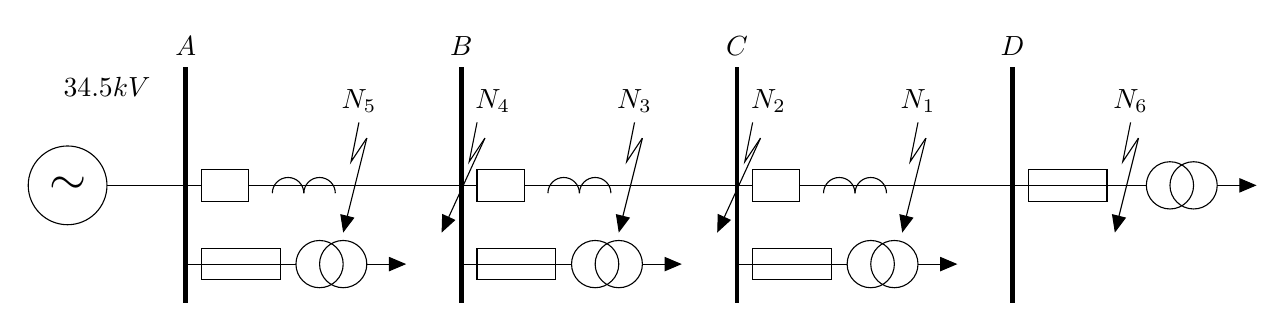
\begin{tikzpicture}[>=triangle 45]
		\draw (0,0) circle (.5)  node{\LARGE{$\mathbf{\sim}$}}; \draw (0.5,1) node[above] {$34.5kV$};
		\draw (0.5, 0) -- (1.5,0);
		\draw[ultra thick] (1.5,1.5) node[above]{$A$} -- (1.5, -1.5);
		\draw (1.5,-1) -- (2.9,-1); \draw (1.7,-.8) rectangle (2.7,-1.2); \draw (3.2,-1) circle (.3); \draw (3.5,-1) circle (.3); \draw[->] (3.8,-1) -- (4.3,-1);
		\draw (1.5, 0) -- (1.7, 0); \draw (1.7, .2) rectangle (2.3,-.2); \draw (2.3,0) -- (5,0); \draw (3,-0.1) arc (0:180:0.2); \draw (3.4,-0.1) arc (0:180:0.2); \draw (3.7, .8) node[above]{$N_5$} -- (3.6,0.3) -- (3.8,0.6);\draw[->] (3.8,0.6) -- (3.5,-.6);
					
		\draw[ultra thick] (5,1.5)node[above]{$B$}  -- (5, -1.5);
		\draw (5,-1) -- (6.4,-1); \draw (5.2,-.8) rectangle (6.2,-1.2); \draw (6.7,-1) circle (.3); \draw (7,-1) circle (.3); \draw[->] (7.3,-1) -- (7.8,-1);
		\draw (5, 0) -- (5.2, 0); \draw (5.2, .2) rectangle (5.8,-.2); \draw (5.8,0) -- (8.5,0);  \draw (6.5,-0.1) arc (0:180:0.2); \draw (6.9,-0.1) arc (0:180:0.2);  \draw (7.2, .8) node[above]{$N_3$} -- (7.1,0.3) -- (7.3,0.6);\draw[->] (7.3,0.6) -- (7,-.6); \draw (5.2, 0.8) -- (5.1, 0.3) -- (5.3,0.6); \draw[->] (5.3, 0.6) -- (4.75,-.6); \draw (5.4,0.8) node[above] {$N_4$};
					
		\draw[ultra thick] (8.5,1.5) node[above]{$C$}  -- (8.5, -1.5);
		\draw (8.5,-1) -- (9.9,-1); \draw (8.7,-.8) rectangle (9.7,-1.2); \draw (10.2,-1) circle (.3); \draw (10.5,-1) circle (.3); \draw[->] (10.8,-1) -- (11.3,-1);
		\draw (8.5, 0) -- (8.7, 0); \draw (8.7, .2) rectangle (9.3,-.2); \draw (9.3,0) -- (12,0);  \draw (10,-0.1) arc (0:180:0.2); \draw (10.4,-0.1) arc (0:180:0.2);  \draw (10.8, .8) node[above]{$N_1$} -- (10.7,0.3) -- (10.9,0.6);\draw[->] (10.9,0.6) -- (10.6,-.6);   \draw (8.7, 0.8) -- (8.6, 0.3) -- (8.8,0.6); \draw[->] (8.8, 0.6) -- (8.25,-.6); \draw (8.9,0.8) node[above] {$N_2$};
					
		\draw[ultra thick] (12,1.5) node[above]{$D$}  -- (12, -1.5);
		\draw (12,0) -- (13.7,0); \draw (12.2,.2) rectangle (13.2,-.2); \draw (14,0) circle (.3); \draw (14.3,0) circle (.3); \draw (13.5, .8) node[above]{$N_6$} -- (13.4,0.3) -- (13.6,0.6);\draw[->] (13.6,0.6) -- (13.3,-.6); \draw[->] (14.6, 0) -- (15.1,0);
	\end{tikzpicture}
\end{document} 